\chapter{Gain}
\label{chap:gain}

\section{Gain Calibration}
To ensure that reconstructed energy is accurate, the detector requires a pixel-level calibration. This calibration is required both for noise and gain. In this section we will see how it is possible to calibrate non uniform gain response of the readout chip.

There are two possible method to calibrate the gain. All of them require a monochromatic source, to know exactly the number of electrons produced by the incident photon. The first method uses only one-pixel events. This condition imposes that all the charge has been deposited in a single pixel, thus we can estimate the gain of the pixel as $g_{ij} = ADC_{ij} / n_e$, where $n_e$ is the number of electrons produced by the photon, which is $E_0 / 3.6$ eV (for silicon sensor). Considering the statistical nature of the ionization process, which introduces an uncertainty in $n_e$, which is distributed according to a Gaussian, we can calculate the mean value $\bar{g}_{ij} = 1/N\sum_k g_{ij, k}$. To have success in the estimate of the gain, we need a high number of one-pixel events. But we know that this type of events is less than a third of all the events. Considering the dimension of the chip, which consists of ~100000 pixels, in order to have a sufficient statistic we would need an impressive amount of events, and we would throw away the majority of them. This is still possible, but it would not be efficient to not consider most of the events. Using simulated dataset, this method shows a negative bias in the gain distribution. This is due to the zero suppression threshold applied to the clustering. It is not possible to use a zero threshold, because the noise is high enough to always contaminate the signal, and without applying a threshold the number of good events would be smaller. On the other hand, this method has very short tails.

The second method allows to use all of the good events (the events accepted after the clustering process, which are one, two and three pixel events). It relies on the assumption that all of the charge of an event is deposited the cluster pixels, and the sum of the charge is equal to the total number of electrons produced by the photon $E_0 - \sum_{i,j} ADC_{ij}/g_{ij}  = 0$. This is independent of the number of pixels involved in an event. The estimation of the gain values is then performed with the least squares method, where we are minimizing the quantity:
\begin{equation}
    \chi^2 = \sum_k E_0 - \sum_{ij}ADC_{ij,k}/g_{ij},
\end{equation}
and we have a parameter for each pixel.
This method allows to increase the number of pixels involved in the estimation, improving both the accuracy and the number of parameters estimated. We are not throwing away any good event, and we are using all the information of each event.
This method presents a bias too, but is smaller than the previous method. The distribution has also a smaller FWHM, but the main problem is the presence of long tails and evident bad estimated parameters, in particular on the boarder of the illuminated region. (Note for the analysis: we can see if we can get the uncertainty of the parameters and throw away the pixels with a big uncertainty, knowing that they are not good estimates.) We can impose a cut on the number of events for each pixel, which is not too strong as would be for the previous method. 

The following steps should be: understand the relation between the distribution properties and the suppression threshold (if the distribution becomes broader), understand if we can manually shift the values after the fit and how it behaves with increasing noise. We should also understand if the estimate is independent of the value of the gain and the pattern (in other words, understand the correlation between neighbor pixels).

There are some fixes to do for the second method, but it is with no doubt the best method. We can see that the number of events per pixel scales with $3N/n_{pix}$ total number of events, which means that it is easy to accumulate enough statistics to do a good fit for the majority of the pixels (e.g if N = $10^5$, $n_{pix} =1500$, we have around 180 events per pixel, while with the first method the average is 1.5 events/pix). For the first method it scales with a very low power of N.

To conclude, the first method is a good estimator of the gain if we have a few events. The bias is a bit larger than the lsq, but it is still good. The second method is the best method when we have a large number of events. I expect that for all the chip, with about 10 millions of events we can perform a very good gain calibration. 

I should see more carefully the way I'm cutting bad results with the signal power of the lsq.

The real test for the goodness of the gain resolution is the energy reconstruction. We should see a spectrum with a broadening caused by the Fano factor.

We should understand if correcting the bias from the reconstructed energy instead of comparing the residuals with a MC reconstruction returns the same results or if there are some differences. I think that doing the bias correction on the reconstructed energy adds a difficult step, which is what is the correct threshold to set for the reconstruction?

\section{Studying the bias dependence on the S/N}
I'm applying the following procedure: we have a dataset with non-uniform gain response, with a certain S/N ratio. We calculate a first estimation of the gain map, but we know that there is a bias in the residuals (We still need to understand the role of the zero suppression in this step, for now we are setting it at 1 sigma ENC). To correct the bias, we run a simulation with the same S/N but with uniform pixel response. We should find a way to correctly show that the bias is independent of the pattern of the gain map, thus we obtain the same bias on the residuals. At this point, we fit the residuals hisotgram with a gaussian to find the center and then we can apply the correction to the gain. After this we can reconstruct the event as usual.

ATTENTION: in this step we don't want to reconstruct the exact eneergy of the line. Our goal is to match the reconstruction that we would perform with the monte carlo gain map. We don't want to fix the bias using the energy of the line, but we need to use the mean reconstructed energy for a given zero suppression threshold. The correction with the residuals seems to be a good method to match this reconstruction.


Considering that the bias depends on the value of the gain, we cannot use a uniform map with 1. I tested a method that seems to work. We calculate the first estimate of the gain, then we create a unform map with gain set to the mean of the previous map. We run a simulation with that map and reconstruct the gain. We calculate the residuals and fit with a gaussian to find the bias. Then we apply the correction to the first gain map. This method seems to work with high S/N. 

\begin{figure}
    \centering
    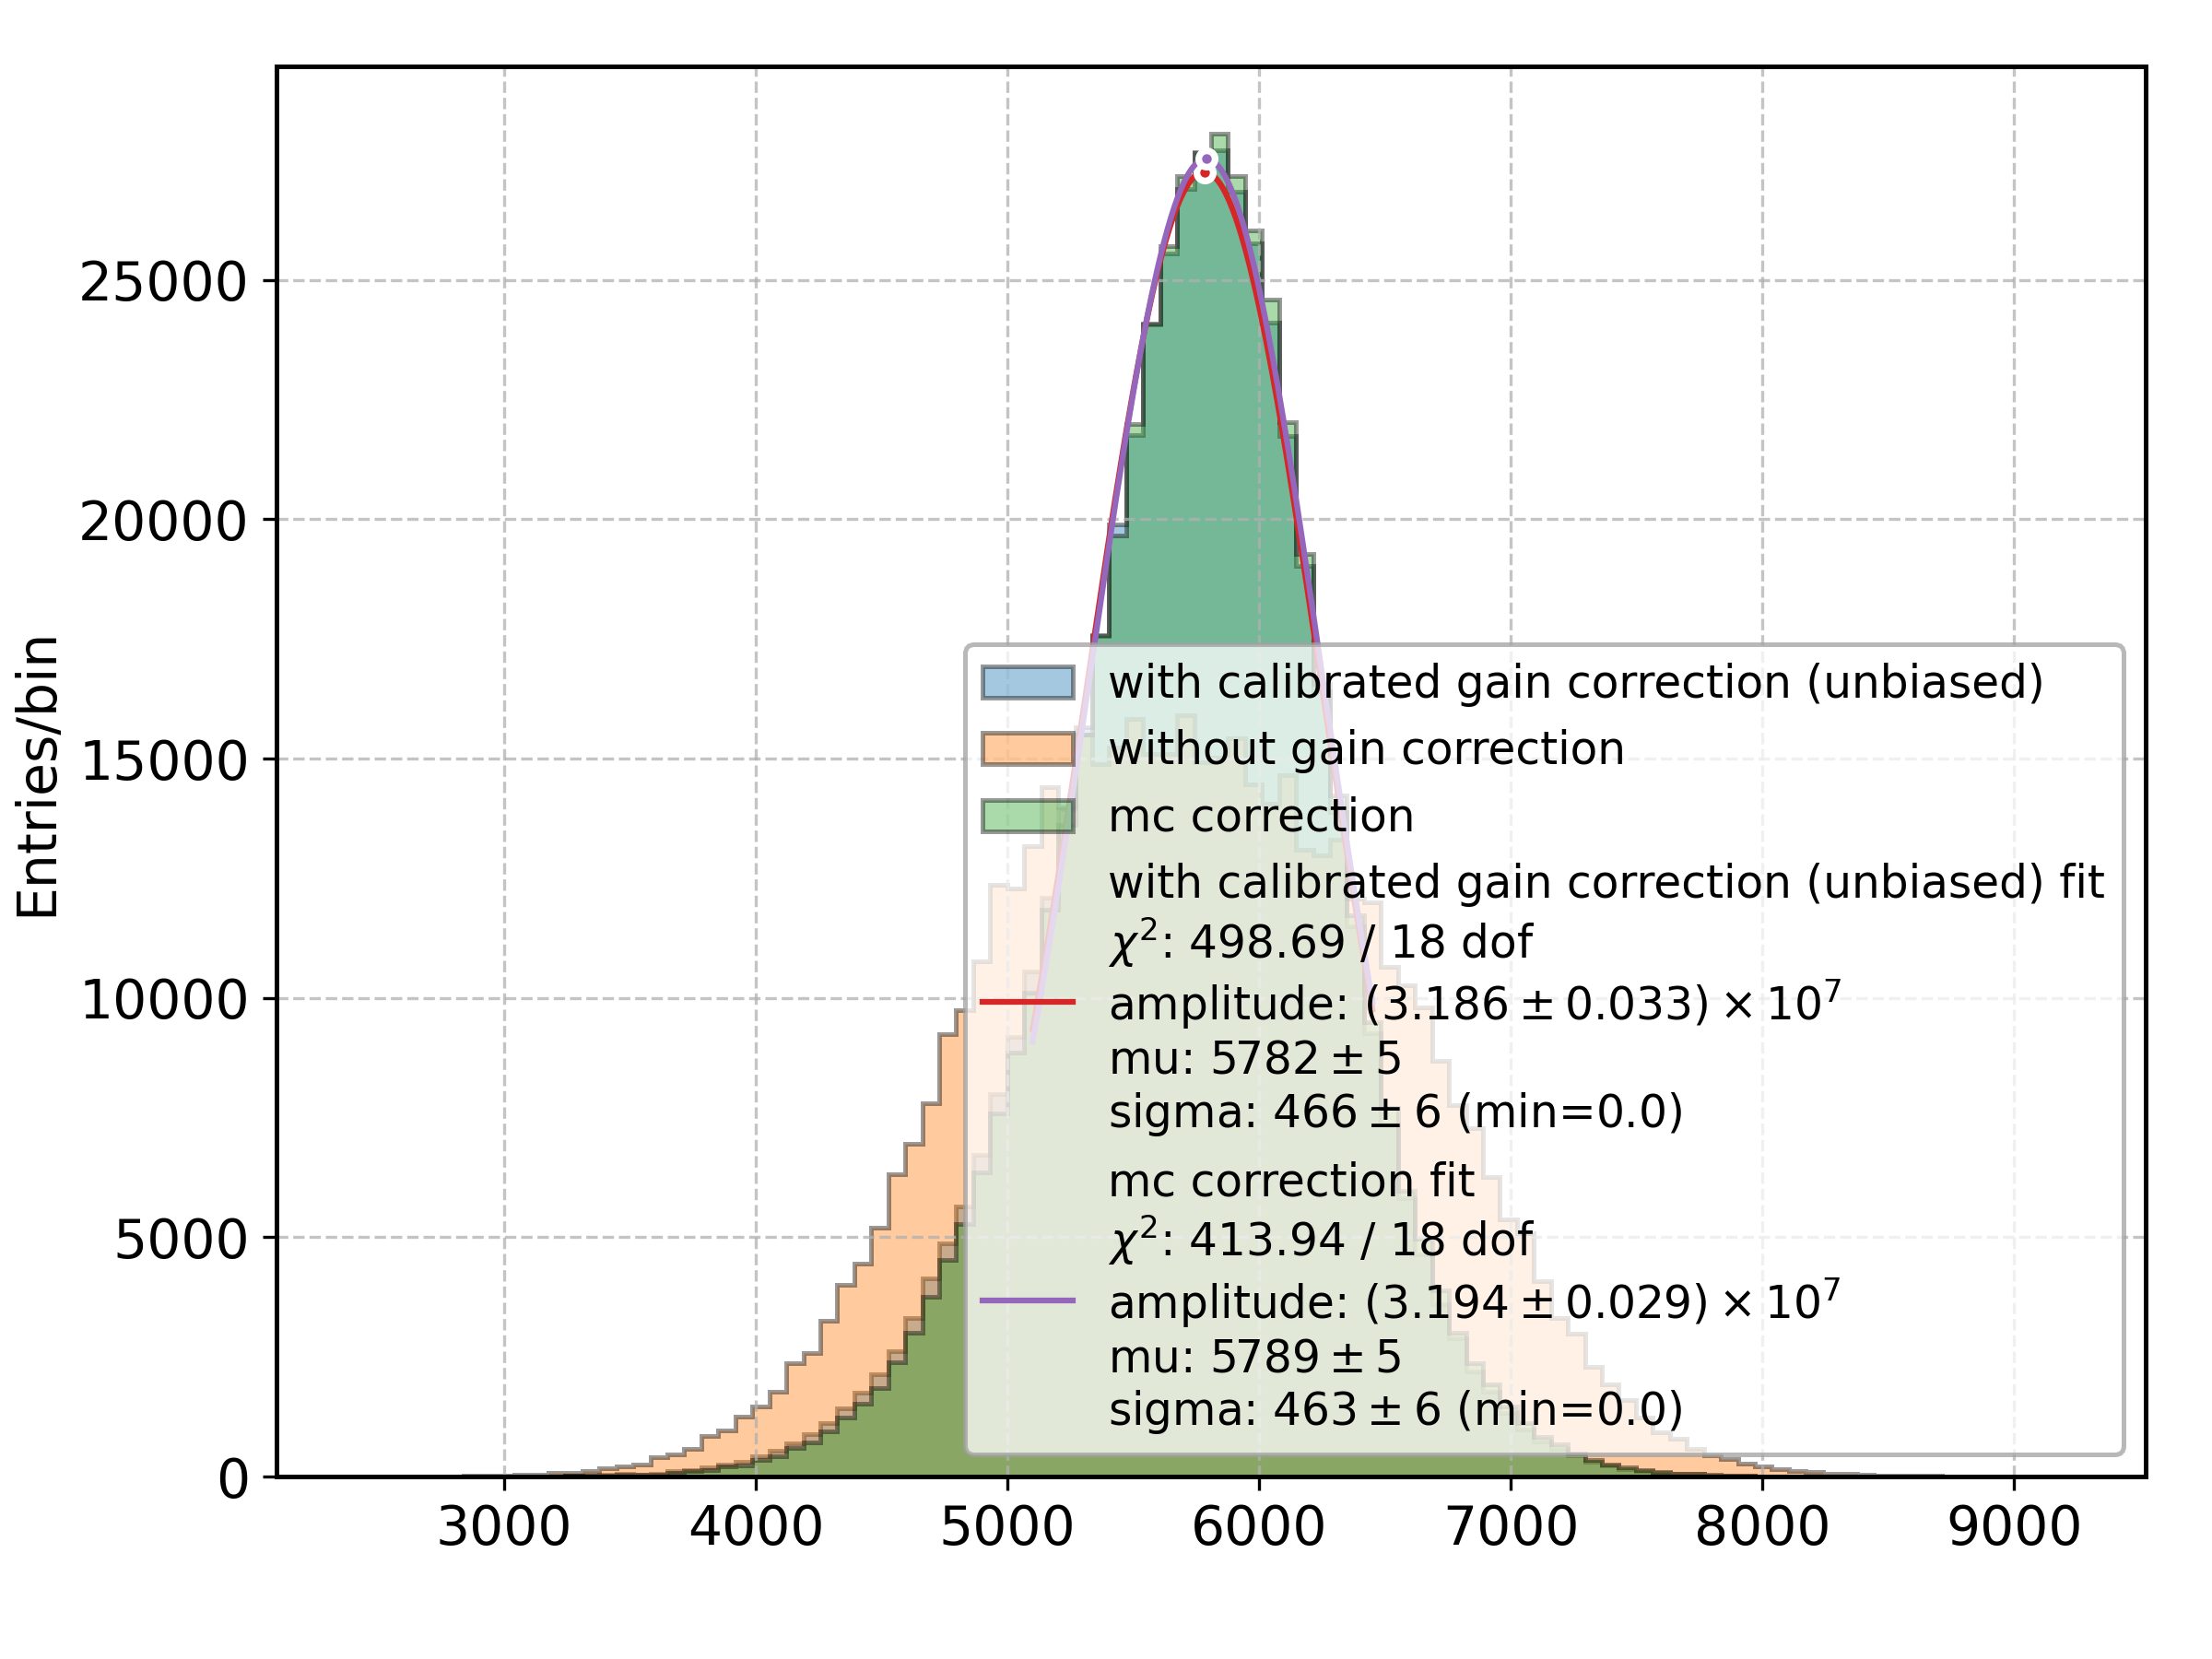
\includegraphics[width=\linewidth]{figures/gain_recon.png}
    \caption{This plot shows the reconstructed spectra in the 3 cases: with no correction, with mc correction and with calibrated correction. The simulation is performed with SNR 20, 6 keV, 500000 events, 3 sigma of zero sup in all the steps (calibration and reconstruction). We can see that the mc and calibrated correction are identical, so the method works. We still need to find a way to justify some choices.}
    \label{fig:enter-label}
\end{figure}

Questions:

Do we expect a dependence of the gain on the energy of the photon? My guess is that this is not the case, as there is no charge multiplication step in the detector.

How can we justify taking the mean of the map? And also how can we demonstrate that there is no dependence on the gain distribution (e.g. it doesn't have to be symmetrical around the mean value).

We should also check which variation can we detect with this method, e.g. if taking the mean is good also if there is a 40\% variation of the gain (I)


\newpage
\section{Gain (good version)}
The first step to correctly reconstruct the energy of the events is to characterize the gain response of the readout chip. This characterization has to be performed for each pixel, otherwise the assumption that the gain response is uniform all over the chip could lead to an error in the reconstructed energy.

This characterization is commonly performed using a monochromatic source with know energy that uniformly illuminates the chip. Knowing the energy of the photons, the mean number of electrons produced can be estimated and using the ADC value of the pixels the gain can be computed. However, the geometry and readout logic of the detector require more caution. It must be noted that one of the feature of the detector is the charge sharing between the pixels, and this implies that it is not possible to directly calibrate each single pixels using all the events. This would require that only one-pixel events should be used for this task, but the number of these events would be about a third of the total number of events, meaning that the remaining events would be thrown away, with the result of being a very inefficient procedure.

The obvious solution is to use all of the events, in order to keep all the information. To find the best procedure to determine the gain, we can start with the assumption that all the charge produced by the photon is collected by the pixels that are being analyzed. This has a consequence on the final result, but it will be later discussed and solved (so we are ignoring the zero-suppression consequences). For a single event, the probability density function of the charge collected by all the pixels is a Gaussian distribution

\begin{equation}
p(\vec{q}; \vec{w}) = \frac{1}{\sqrt{2\pi}\sigma} \exp{\left(-\frac{(\vec{q}\cdot \vec{w} - E_0)^2}{2\sigma^2} \right) },
\end{equation}

where $\vec{q}$ and $\vec{w}$ denote the charges of the pixels and the inverse of the gain, respectevely, and $\sigma^2$ is the variance of the distribution, that has contributions from both the noise and the statistical fluctuations of the number of charges produced by the photon. It follows that when considering all the events, the negative log-likelihood, ignoring the constant, is the usual $\chi^2$

\begin{equation}
- \log \mathcal{L}(\vec{w}) = \sum_i \frac{(\vec{q}_i \cdot \vec{w}_i - E_0)^2}{2\sigma^2} + \textrm{const}.
\end{equation}

To find the best-fit parameters, we find the minimum of the $\chi^2$, that is


\begin{equation}
\frac{\partial \chi^2}{\partial w_{\alpha \beta}} = \sum_i \frac{(\vec{q}_i \cdot \vec{w}_i - E_0)}{\sigma^2} \frac{\partial(\vec{q}_i \cdot \vec{w}_i)}{\partial w_{\alpha \beta}} = 0,
\end{equation}

where $\vec{w}_i$ is the vector containing the inverse of the gain for the pixels in the $i$-th event, and $\vec{w}_{\alpha \beta}$ is the invers of the gain of the pixel in the $\alpha$-th row and $\beta$-th column. This equation means that we have to find the the best values of $w$ such as

\begin{equation}
w_{fit} = \textrm{arg min} ||Qw - E_0 ||^2
\end{equation}

where $Q$ is the matrix containing the charge collected by all the pixels of the readout chip for all the events, while $w$ is the vector of the pararameters to find and $E_0$ is the vector of the known value.

Due to the fluctuations in the number of electrons produced by the interactions and the effect of electric noise on the pixels, it is required to have a large number of events for each pixel we want to calibrate.

The main problem in the gain calibration process, is that we need to distinguish between the pixels that only have noise and the ones that have signal. This step requires the same procedure used for the position reconstruction, which consists in setting a zero suppression level, setting pixels below that value to zero, taking at most three pixels per event and checking that all of them are neighbors. The zero suppression is the difficult step, because even if it reduces the noise, it can also remove some signal charge, and the overall effect is that the real charge used for the fit is less than that produced by the photon, with the result of underestimating the gain.

\subsection{Calibration procedure}
After simulating a file with a certain signal-to-noise ratio, a monochromatic source and a pixel gain response distrubuted according to a known distribution, the first step of the calibration is to run a first fit on the data, to have a first estimate of the gain. This steps requires to set a zero-suppression threshold to cut pixels dominated by noise, and a check on the position of the pixels is also performed, in the same way is done for the position reconstruction. As previously mentioned, the zero-suppression introduces a bias in the gain estimate, because some of the signal charge is thrown away. To estimate the level of bias, a new set of events is simulated, this time using the best-fit pixel gain response, and with the same SNR and energy of the first file. On this new simulation, the same calibration procedure as before is performed. The goal is to compare the best-fit gains obtained for the second simulation with the best-fit gains obtained from the first file, that in this case is a simulation, but in the future it will be the real data.

Knowing the pixel gain response matrix used for the second simulation, it is possible to compare the results and calculate the residuals. The mean of the residuals distribution gives the bias $b$ of the calibration. Using this information, the first best-fit gain response matrix can be scaled to compensate the bias

\begin{equation}
g_{unbiased}   = \frac{1}{1 + b} g_{biased}.
\end{equation}

\subsection{Calibration evaluation}
To assess the goodness of the calibration procedure, different simulations have been made using a known gain response matrix, distributed according to a Gaussian distribution

\begin{equation}
g \sim \textrm{Gauss}(g; \mu = 0.08, \sigma = 0.01),
\end{equation}

which reflects the expected distribution on the real readout chip. The monochromatic source energy is set to 10 keV, approximately the same energy of a Au target, and the SNR is set to 20, meaning that the noise distribution has a standard deviation of about 135 e$^-$, which is a bit more pessimistic than the real data. To ensure the fit can converge to the right value, the number of events per pixel sould be quite large. For this simulation, $5\times 10^5$ events have been simulated over a circle qith a $0.15$ cm radius, meaning that about 3000 pixels are contained in the area. The mean number of times that a pixel is over threshold is about 200, which is enough to correctly perform the fit. Increasing this number would result in a higher accuracy of the gain estimate, because it compensates the effects of the electric noise and the statistical fluctuations of the produced number of electrons.

!!! I SHOULD DECIDE WHETHER TO KEEP FIG \ref{fig:gain_distribution} OR CHANGE IT WITH THE DISTRIBUTION OF THE RESIDUALS, WHICH IS MORE MEANINGFUL !!!

Fig. \ref{fig:spectra} shows the energy spectra reconstructed with the Monte Carlo gain response matrix, with the best-fit matrix and with the same value of the gain for all the pixels. From the figure, it is evident that the assumption of a uniform gain response is not good for this dataset. The results depend on the variance of the distribution. The larger the dispersion of the gain values, the worse the reconstructed spectrum is.


\begin{figure}
    \centering
%    \includegraphics[width=0.8\linewidth]{figures/gain/gain_distribution}
    \caption{Comparison between the Monte Carlo pixel gain distribution and the best-fit gain distribution. These distributions only contain the value of the pixels contained in a disk beam with a radius of 0.15 cm, which are about 3000 pixels.}
    \label{fig:gain_distribution}
\end{figure}

\begin{figure}
    \centering
    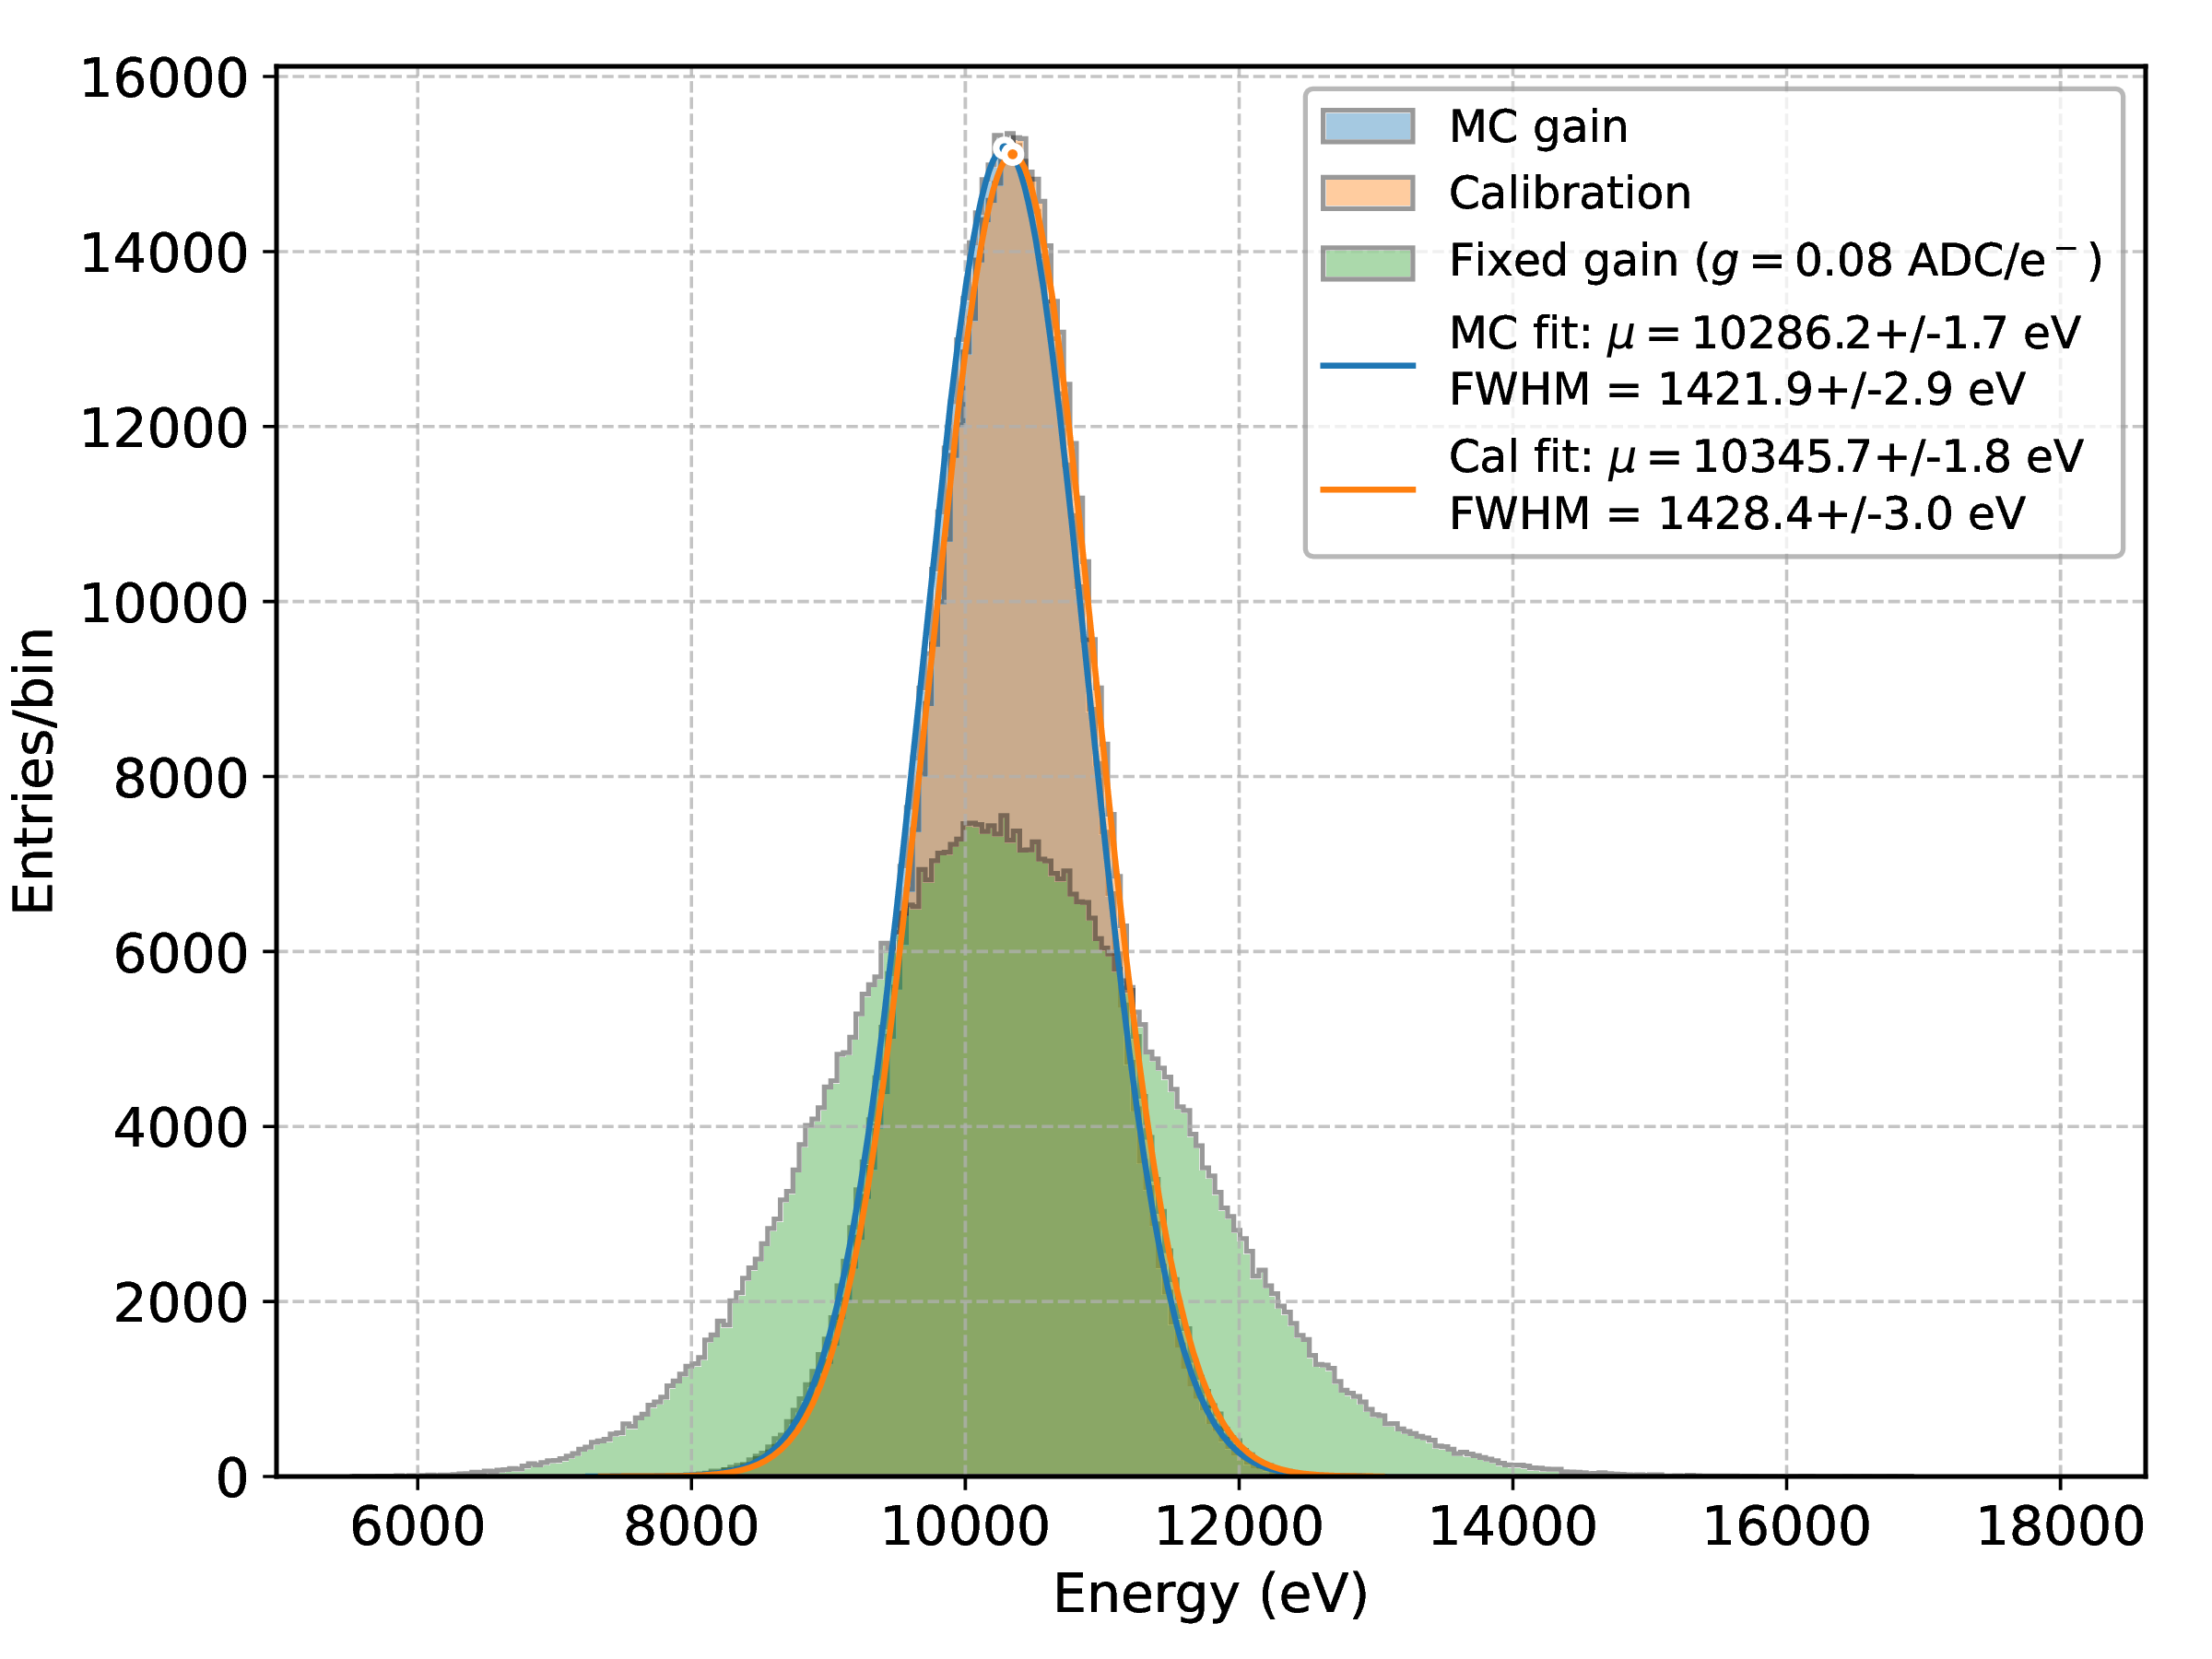
\includegraphics[width=0.8\linewidth]{figures/gain/spectra}
    \caption{Reconstructed energy spectra of the simulated monochromatic source of 10 keV. In green, the spectrum reconstructed assuming that all the pixels have the same gain $g = 0.08$ ADC/e$^-$. In blue, the spectrum reconstructed with the true Monte Carlo pixel gain response matrix with the respective Gaussian best-fit curve. In orange, the spectrum reconstructed with the best-fit pixel gain response matrixm, along with the respective Gaussian best-fit curve.}
    \label{fig:spectra}
\end{figure}


\subsection{Real data}












